\documentclass[a4paper,10pt]{jsarticle}

% 数式
\usepackage{amsmath,amsfonts}
\usepackage{bm}
% 画像
\usepackage[dvipdfmx]{graphicx}
\usepackage{here}

\usepackage{listingsutf8,jlisting} %日本語のコメントアウトをする場合jlistingが必要
%ここからソースコードの表示に関する設定
\lstset{
  basicstyle={\ttfamily},
  identifierstyle={\small},
  commentstyle={\smallitshape},
  keywordstyle={\small\bfseries},
  ndkeywordstyle={\small},
  stringstyle={\small\ttfamily},
  frame={tb},
  breaklines=true,
  columns=[l]{fullflexible},
  numbers=left,
  xrightmargin=0zw,
  xleftmargin=3zw,
  numberstyle={\scriptsize},
  stepnumber=1,
  numbersep=1zw,
  lineskip=-0.5ex
}

\begin{document}

\title{ソフトウェア設計法レポート\\添削希望}
\author{坪井正太郎(101830245)}
\date{\today}
\maketitle
前回のレポートを提出していないので、大学の成績システムを想定した。
講義を担当する教員が成績を入力し、それを学生が参照する。
また、学務は成績の情報から進級条件を満たしているかチェックする。

\section{ユースケース図}

\begin{figure}[H]
  \centering
  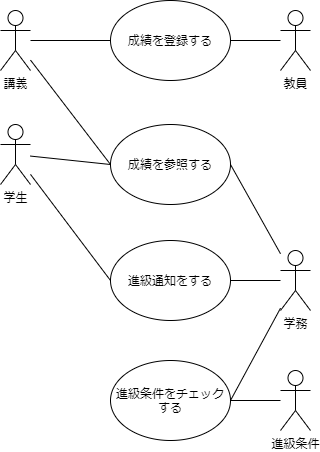
\includegraphics[width=8cm]{./01.drawio.png}
  \caption{ユースケース図}
  \label{ユースケース図}
\end{figure}

\section{イベントフロー}
\subsection{成績を登録する}
\begin{enumerate}
  \item 事前条件
  \item 基本フロー\\
        教員は、成績をつけたい講義と、学生を選択する。その後、SABCFのいずれかの成績を選択する。すべての学生に成績をつけ、登録する。[E-1]
  \item 例外フロー\\
        E-1:受講生の中で、成績がつけられていない学生がいる場合、警告を表示する。
\end{enumerate}

\subsection{成績を参照する}
\begin{enumerate}
  \item 事前条件
  \item 基本フロー\\
        学生、または学務は、講義を選択する。画面上に成績が表示される。[E-2]
  \item 例外フロー\\
        E-2:成績の公開期間に入っていない場合、未公開であるという表示を出す。
\end{enumerate}

\subsection{進級条件をチェックする}
\begin{enumerate}
  \item 事前条件
  \item 基本フロー\\
        学務は、進級条件と成績から、進級が可能かどうか調べる。
  \item 例外フロー
\end{enumerate}

\subsection{進級通知をする}
\begin{enumerate}
  \item 事前条件
  \item 基本フロー\\
        学務は、学生の進級が可能かどうか調べ、結果を登録する。
        進級が不可となった学生には、通知を行う。
  \item 例外フロー
\end{enumerate}


\end{document}
